\documentclass[12pt,a4paper]{article}
\usepackage[left=2cm,right=2cm,top=3cm,bottom=3cm]{geometry}
\usepackage{graphicx} %%
\usepackage{epsf,epstopdf}
\usepackage[dvipsnames]{xcolor}
\usepackage{tikz}
\usetikzlibrary{shapes,arrows}
\usepackage{amsmath,amsthm,amsfonts,amscd,amssymb,bm}
% \usepackage{verbatim}
\usepackage{hyperref}
% \usepackage{CJKutf8,CJKnumb,CJKulem}
\usepackage{fancyhdr}
\usepackage{multirow}
% \usepackage{array,ulem}
% \usepackage{cancel}
% \usepackage[explicit]{titlesec}
\usepackage{cite}
\usepackage{indentfirst}


\begin{document}

\title{\textbf{Stirring by anisotropic squirming}\vspace{0.5em}}
\author{ZHI LIN$^{a}$\thanks{Corresponding author. Email address: linzhi80@zju.edu.cn (ZHI LIN)}\vspace{-2em}}
\date{\vspace{-3em}}
\maketitle
\begin{center}
  \small\textsl{$^{a}$School of Mathematical Sciences, Zhejiang University,
    Hangzhou, Zhejiang 310027, China}\\[50pt]
\end{center}
\rule[0.25\baselineskip]{\textwidth}{1pt}

\section*{\normalsize{Abstract}}

\noindent
In this paper,
we consider a fluid stirred by the locomotion of submerged swimming bodies,
we generalize the model proposed by Thiffeault and Childress\cite{Stirr}
and study swimmers moving in anisotropically random directions.
The stirring-induced, anisotropic effective diffusion tensor is calculated
from the classical It\^o theory in 2D and in axisymmetrically 3D,
respectively. We defined two dimensionless scalar indices to
quantify the anisotropy in the diffusive process.
Further, we found that given different probability distributions,
the different anisotropic stirring may cause the same diffusion property.
With comparing the analytical result of diffusion tensor of particle and swimmer,
we found a number which measures the difference between them.
Next we studied the relationship between the anisotropy of swimming and that of diffusion coefficient,
and proposed two dimensionless numbers which measure the two anisotropy respectively. From those numbers we can easily judge the anisotropy of them.\vspace{0.75em}

\noindent
\textsl{Keywords:} biomixing, diffusion tensor, anisotropic,
distribution\vspace{0.75em}

\noindent
\rule[0.25\baselineskip]{\textwidth}{1pt}

\section*{\normalsize{1. Introduction}}

In the past two decades,
the study of biogenic mixing has attracted a plethora of research efforts.
For scientists and engineers working with swimming organisms submerged in fluid environments of various scales, such as bacteria, algal cells, krill, fish, etc.,
a common and intriguing question frequently arises:
does the collective swimming motion of aquatic species enhance passive scalar mixing?
Especially, this was suggested as a significant mechanism in ocean mixing \cite{Role, Observe},
although its efficiency is still controversial \cite{Do, Biomix, Influ, Turbu}.
Biomixing is biochemical suspensions of small organisms has also been studied
\cite{Enhance, Dynamics, Fluid, Self-conce} for different
experimentally controlled concentrations.

Among the different approaches trying to tackle the problem,
Thiffeault and Childress \cite{Stirr} developed a microscopic framework that
combines the classical results in hydrodynamics and stochastic modeling
and proposed a rigorous formula for effective diffusivity.
The central idea involved is called Darwinian drift,
studied in the pioneering work by Maxwell \cite{OnThe} and Darwin \cite{Onthedispacement}.
It is the mass displacement due to a moving body
and suggested by Katija \cite{Aviscosity} as the dominant effect in the swimming-induced mixing.
Several studies measure drift volume to
directly evaluate the transport ability of an individual swimmer \cite{Drift, FluidDispace, Fluidtransport}.
Alternatively,
in this paper
we follow the methodology by Thiffeault and Childress
since the effective diffusivity computed by averaging multiple drifts
is a natural characterization for the mixing effect of an ensemble of
random swimmers similar to Brownian motion.
Furthermore, it enables us to compare the mixing behavior of a passive scalar
under different physical scenarios documented in a vast spectrum of literature.

Thiffeault, Childress \cite{Stirr} derived the effective diffusivity
of a randomly distributed non-interacting swimmers in potential flows,
and showed that it is due to the repeated displacements induced by a
swimmer on a particle of fluid. Zhi Lin et al. \cite{squirments}
developed this model into stokes flow, given the drift caused by one
swimmer, an effective diffusivity coefficient could be computed. And
those models have been tested in physical experiments and numerical
simulations \cite{EnhancedDiffusion, Induced}. Kasyap et
al. \cite{Hydrodynamic} studied slender-body bacteria affecting the
passive tracers with a similar model and analyzed the dimensionless
number like Peclet number and the diffusion coefficient.

Those models above focused on the isotropic case,
but the anisotropic is more ubiquitous in the nature.
The study of the anisotropic case has many applications,
like designing requisite nanomotors
\cite{SelfPropelling}, manipulating microscale structures which is an
unsolved challenge in microengineering and microtechnology and herding
bacteria, making it move in certain direction, which is one way to achieve
that \cite{Bacterial}. Also for interest in the dynamical properties
of interacting, self-propelled organisms which have tropism movement
under anisotropic fluid \cite{Bacterial} or external field have been
studied \cite{Concentration, Enhance, SwimStress}.
Furthermore, there has a significant different result induce by anisotropic squirming,
which we will discuss in the following sections.

Our paper is constructed as follow. In section 2, we generalize the
model proposed by Thiffeault, Childress \cite{Distribution} into
anisotropic case. In section 3, we propose a general steps to
calculate the effective diffusion tensor of particle by applying Ito
diffusion theory. In section 4, we give a theoretical analysis about
the difference between diffusion tensor of particle and diffusion
tensor of swimmer. In section 5, diffusivity in any given direct in 2
and 3 dimension is calculated. In section 6, we propose the indicator
of anisotropic distribution and indicator of diffusion coefficient in
2 dimension. Section 7 is devoted to comparing our predictions to the
results of numerical simulations.

\section*{\normalsize{2. Stochastic stirring model}}

The setting of our problem is a large volume $V$ that contains a number
of swimmers $N$, also typically large. The swimmers move a distance $\lambda$
independently of each other in random directions and change the
directions randomly. We assume the distribution of swimmers are dilute
enough so that the velocity field of one swimmer is not significantly
affected by the others. Hence a fluid particle (not too near the edges
of the domain), will be displaced by the cumulative action of the
swimmers.

For simplicity, we assume the swimmer start from the original point,
move along straight paths $\lambda$ at a fixed speed $\bm U$. The velocity field
induced at point $x$ by a swimmer is $\bm u(\bm x-\bm{U}t)$. For a fluid particle
which initially at $\bm{x}=\bm{\eta}$ which has uniform distribution in the space
affected by a single swimmer described above, the drift of it is
$\Delta_{\lambda}(\bm \eta,\bm U)$:
\begin{equation}
  \label{eq:1}
  \begin{aligned}
    \Delta_{\lambda}(\bm\eta,\bm U)&=\int^{\lambda/U}_{0}\bm{u}(\bm{x}(s)-\bm{U}s)\
    \mathrm{d}s\\
    \dot{\bm{x}}&=\bm{u}(\bm{x}-\bm{U}t)\\
    \bm{x}(0)&=\bm{\eta}\\
    U&=|\bm{U}|
  \end{aligned}
\end{equation}

Actually, under those equations above, $\Delta_{\lambda}$ do not depend on the
magnitude of $U$. Hence, to introduce a unit vector
$\bm{a}=\frac{\bm{U}}{U}$, which is characterizing the orientation of
the swimmer motion. Let the PDF of swimmers' moving direction be
$f(\bm{a}$. By the definition of $f(\bm{a})$, we have
$f(\bm{a})=f(c\bm{a})$ for any positive constant. We obtain the
probability density of displacement:
\begin{equation}
  \label{eq:2}
  p_{\bm{R}^{1}_{\lambda}}(\bm{r})=\int_{S^{d}}f(\bm{a})\int_{\Omega}\delta(\bm{r}-\Delta_{\lambda}(\bm{\eta},\bm{U}))\
  \frac{\mathrm{d\bm{\eta}}}{V}\mathrm{d}\bm{a}
\end{equation}
Hence $\Omega$ represent the region and $V$ is the area of it,
$\bm{R}^{1}_{\lambda}$ is a random variable that gives the displacement of
the particle from its initial position after being affected by a
single swimmer with path length $\lambda$. We denote by
$p_{\bm{R}^{1}_{\lambda}}(\bm{r})$ the pdf of $\bm{R}^{1}_{\lambda}$, $S^{d}$ is
unit sphere in $d$ dimensions $\bm{R}^{N}_{\lambda}$ represent the
displacement of the particle from its initial position after being
affected by N swimmers with path length $\lambda$. Obviously
$\bm{R}^{N}_{\lambda}=\sum_{i=1}^{N}\bm{R}^{1}_{\lambda}$, according to the dilute
assumption.

\section*{\normalsize{3.Effective diffusion tensor}}

Isotropic case is a kind of perfect state. However, in reality,
anisotropic stirring is more common, like the self-propelled organisms
which has tropism movement under anisotropic fluid \cite{Bacterial},
chemical gradients \cite{Concentration} or external field
\cite{Enhance, SwimStress}, like the anisotropic swimming cause by
stratified structure of ocean \cite{BiogenicInputs}. The anisotropic
stirring make diffusion tensor anisotropic, that is, different
"stirring" effects in different directions. Obviously, if the
probability of swimmers moving along $x$ direction is more than that
of $y$ direction, the effective diffusivity along $x$ direction should
also be bigger than that of $y$ direction, which are always equal in
isotropic case.

There is no doubt that the trajectory of swimmer is equivalent to
Brownian motion on large spatiotemporal scales. But the trajectory of
particle is not exactly too. Those long jump in the figure \ref{fig:1} is due to
heavy tail of pdf. Many article indicated that the pdf has the feature
of Gaussian core and exponential tail \cite{Distribution, Dynamics},
in the experimental and theoretical. On the other hand, the variance
of this process is still proportional to the square of time
\cite{ParticleDiffusion}, which is as same as Brownian motion. In
addition, many article use the effective diffusivity to measure the
effect of stirring \cite{Stirr, DiffusionColloidal}. Therefore, we
still use the effective diffusivity to measure the effect of stirring.

\begin{figure}
  \centering
  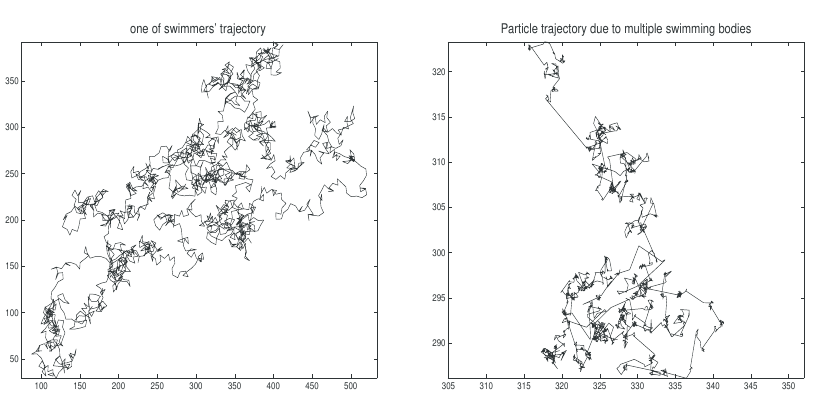
\includegraphics[scale=0.9]{figure1}
  \caption{The plot show the result of numerical simulation. One
    particle is stirred by multiple swimmers, which do the
    run-and-tumble motion. (a) Trajectory of one of those swimmers,
    which is ordinary random walks and is equivalent to Brownian
    motion on large spatiotemporal scales. (b) Particle trajectory due
    to multiple swimming bodies, which exhibits local clustering
    interspersed with long distance jumps. That is feature of heavy tail
    of pdf.}
  \label{fig:1}
\end{figure}

As we discussed above, in the anisotropic case, "stirring" effects in
different directions are different. Hence, it is not enough to
describe the all diffusion ability with one number. We need use the
diffusion tensor instead of it. We use $It\hat{o}$ diffusion process
to describe the trajectory of particle. Now we motion. $It\hat{o}$
diffusion process is the solution to the following stochastic
differential equation:
\begin{equation}
  \label{eq:3}
  \mathrm{d}\bm{R}_{\lambda}(t)=\bm{b}(t,\bm{R}_{\lambda}(t))\mathrm{d}t+\bm{\sigma}(t,\bm{R}_{\lambda}(t))\mathrm{d}\bm{B}_{t},
\end{equation}
where $\bm{R}_{\lambda}(t)\in R^{d},\ \bm{b}(t,x)\in R^{d},\ \bm{\sigma}(t,x)\in R^{d\times
  m}$, $\bm{B}_{t}$ is m-dimensional Brownian motion. $\bm{b}$ is
so-called the drift coefficient and $\frac{1}{2}\bm{\sigma}\bm{\sigma}^{T}$ is
the diffusion coefficient or called diffusion tensor. The displacement
is so small compare to $\lambda$ that we can regard $\bm{b},\ \bm{\sigma}$ as
approximately invariant that have no correlation with time and
space. By straightforward calculating, the expression of the diffusion
tensor show
\begin{equation}
  \label{eq:4}
  DT=\frac{1}{2}\bm{\sigma}\bm{\sigma}^{T}=\frac{\Big(\mathrm{cov}\Big(\bm{R}_{\lambda,i}(t),
        \bm{R}_{\lambda,j}(t)\Big)\Big)_{d\times d}}{2t},
\end{equation}
where $\bm{R}_{\lambda,i}(t)$ is the i-th coordinate component process of
total process $\bm{R}_{\lambda}(t)$. Within one period time $t=\frac{\lambda}{U}$,
the displacement induced by all swimmers in the region is $\bm{R}_{\lambda}^{N}$.
When $\lambda$ is large enough the displacement induced in each period can
be regard as independence and
$\bm{R}_{\lambda}^{N}=\sum_{i=1}^{N}\bm{R}_{\lambda}^{1}$, diffusion tensor become

\begin{equation}
  \label{eq:5}
  \begin{aligned}
    DT&=\frac{U\Big(\mathrm{cov}\Big(\bm{R}_{\lambda,i}^{1},
          \bm{R}_{\lambda,i}^{1}\Big)\Big)_{d\times d}\{DT_{i,j}\}_{i,j}}{2\lambda}\\
      &=\frac{nU\int_{\Omega}\Delta_{\lambda}(\bm{\eta})^{2}\
        \mathrm{d}\bm{\eta}}{2\lambda}\{E\Big(r^{1}_{k,i},r^{1}_{k,j}\Big)
      -\rho E\Big(r^{1}_{k,i}\Big)E\Big(r_{k,j}^{1}\Big)\}_{i,j}.
  \end{aligned}
\end{equation}
Here $r^{1}_{\lambda,i}$ is the i-th component of unite vector which
represent the direction of $\bm{R}_{\lambda}^{1}$, and
\mbox{$\rho=\frac{(\int_{\Omega}\Delta_{\lambda}(\bm{\eta})\ 
    \mathrm{d}\bm{\eta})^{2}}{V\int_{\Omega}\Delta_{\lambda}(\bm{\eta})^{2}\ \mathrm{d}\bm{\eta}}$}.
With the fact that $\rho\to0$, when $V\to\infty$, the \eqref{eq:5} turn out to be
\begin{equation}
  \label{eq:6}
  DT=\frac{nU\int_{\Omega}\Delta_{\lambda}(\bm{\eta})^{2}\ \mathrm{d}\bm{\eta}}{2\lambda}\{E\Big(r^{1}_{k,i},r^{1}_{k,j}\Big)\}_{i,j}.
\end{equation}

The effective mean diffusivity $\kappa$, which we often discussed in the
isotropic case, is average of trace of diffusion tensor. And because
of
$\sum_{i=1}^{d}E(r_{k,i}^{1},r_{k,j}^{1}=E(\sum_{i=1}^{d}r_{k,i}^{1}r_{k,j}^{1})=E(1)=1$:
\begin{equation}
  \label{eq:7}
  \kappa=\frac{1}{d}\mathrm{tr}(DT)=\frac{nU\int_{\Omega}\Delta_{\lambda}(\bm{\eta})^{2}\ \mathrm{d}\bm{\eta}}{2d\lambda},
\end{equation}

From equation \eqref{eq:5}, we know that in finite domain effective
mean diffusivity may smaller when swimmer has orientational drift. On
the contrast, from equation \eqref{eq:7} when the domain is infinite,
the pdf do not influence the value of effective mean
diffusivity. Following those steps in this section we have made,
supposing the pdfs of each random reorientations of swimmers are
different but independent, the effective mean diffusivity still will
not change. In other words, under our assumption of model, the
mechanism of random reorientations is independent of the effective
mean diffusivity. Although the mechanism of random reorientations do
not change the effective mean diffusivity, but it will change the
effective diffusivity in given directions. That is what we will
discuss in the next section.

\section*{\normalsize{4. Diffusion of particle and diffusion of
    swimmers.}}

Swimmers are power source of particles. So the diffusion tensor of
particle should have the relationship with the diffusion tensor of
swimmer. It is easy to get the diffusion tensor of swimmer follow the
same steps of the previous section:
\begin{equation}
  \label{eq:8}
  DTS=NU\lambda\{E\Big(a_{i}a_{j}\Big)\}_{i,j}=NU\lambda\{\int_{S^{d}}
  f(\bm{a})(\bm{a}\cdot\bm{e}_{i})(\bm{a}\cdot\bm{e}_{j})\ \mathrm{d}\bm{a}\}_{i,j}
\end{equation}
$\bm{a}$ is the moving direction of swimmer, and $a_{i}$ is the i-th
component of $\bm{a}$. 

If the direction of swimmer motion and the drift of particle induced
by it are the same, that is, $\bm{r}$ and $\bm{a}$ are
collinear. $DT$, $DTS$ should be proportional. But the relationship
$\bm{r}=C\bm{a}$ is not always true, see figure 2.

In this section, we will calculate $DT$, and then analyze the
difference between $DT$ and $DTS$. Two concrete swimming models will
be analyzed below, stokes flow and planar potential flow. In stokes
flow, we choose a specific instance of an axially symmetric squirmer
of radius $l$, swimming along the positive z-axis at a constant speed
$U$. Its free-space, steady, axisymmetric streamfunction in a comoving
reference frame is:
\begin{equation}
  \label{eq:9}
  \psi(\rho,z)=\frac{1}{2}\rho^{2}U\bigg(-1+\frac{l^{3}}{r^{3}}+\frac{3\beta
    l^{2}z}{2r^{3}}\bigg(\frac{l^{2}}{r^{2}}-1\bigg)\bigg)
\end{equation}
in cylindrical coordinates where
$r=\rho^{2}+z^{2}=x^{2}+y^{2}+z^{2}$. When $\beta=0$, the flow become the 3D
potential flow. In the planar potential flow case, swimmer of radius $l$
\newpage

\bibliographystyle{unsrt}
\bibliography{./ref.bib}

\end{document}
%%% Local Variables:
%%% mode: latex
%%% TeX-master: t
%%% End:
